\section{Systematic uncertainties}
\label{sec:systematics}

% Systematic variations are propagated by rerunning the full unfolding chain for each
% variation and comparing to the nominal unfolded result. For each source $v$, the
% signed bin-wise shift is
% \begin{equation}
% \delta_v(j)=\frac{U_v(j)-U_{\mathrm{nom}}(j)}{U_{\mathrm{nom}}(j)}.
% \end{equation}
% The sources are grouped into seven independent components

Systematic uncertainties arise from several components: data statistical, MC statistical, unfolding-regularization, experimental variations, theory unfolding prior, hadronic event-selection correction, and ISR correction. The sections below describe each component.

\subsection{Statistical uncertainty}
\label{sec:stat_uncertainty}

The data statistical uncertainty is propagated analytically by RooUnfold through the IBU iteration chain, without toy-MC sampling, yielding a full statistical covariance matrix $\mathrm{Cov}^{(\mathrm{stat})}_{ij}$. The per-bin fractional uncertainty $\Delta_{\mathrm{stat}}(j)=\sqrt{\mathrm{Cov}^{(\mathrm{stat})}_{jj}}/U_j^{\mathrm{corr}}$ is typically below $2\%$ in the central range and nearly uniform across the spectrum. The uncertainty is shown in Figure~\ref{fig:unc_comp_stat_iter}.

MC statistical uncertainties enter the budget through the two corrections derived from finite simulated samples: the MC statistical uncertainty of the ISR-off and ISR-on samples is propagated onto $C_{\mathrm{ISR}}(j)$, and the archived-MC statistical uncertainty of $N_{\mathrm{genBefore}}$ and $N_{\mathrm{gen}}$ is propagated onto the hadronic event-selection correction $C_{\mathrm{had}}(j)$. The finite statistics of the response matrix itself are propagated separately, by giving every matched simulated event a Poisson weight and re-unfolding the data over 200 such replicas; the sample covariance of the resulting spectra is taken as $\mathrm{Cov}^{(\mathrm{MCstat})}_{ij}$. This is required because \texttt{RooUnfold::kCovariance} transports the measured data covariance only, and because the simulated sample is smaller than the data sample, so the response statistical term exceeds the data statistical term in every bin.

\subsection{Unfolding regularization uncertainty}
\label{sec:stat_uncertainty}

The unfolding regularization uncertainty is closely related: two additional unfolding passes at $N_{\mathrm{iter}}=4$ and $N_{\mathrm{iter}}=6$ quantify the sensitivity of the result to the regularization choice. The iteration envelope $\Delta_{\mathrm{iter}}(j)=\max(|\delta_{\mathrm{iter4}}(j)|,|\delta_{\mathrm{iter6}}(j)|)$
is sub-percent in the bulk of the spectrum, confirming that the nominal $N_{\mathrm{iter}}=5$ sits on a stable plateau and that regularization is not a limiting source of uncertainty. Figure~\ref{fig:unc_comp_stat_iter} shows the
signed per-bin shifts for both components across the measurement range. The iteration shifts change sign across the range because $N_{\mathrm{iter}}=4$ and $6$ bracket the nominal, and the bin-to-bin alternation at low thrust reflects the anti-correlation that regularization induces between neighboring bins.

\begin{figure}[ht!]
\centering
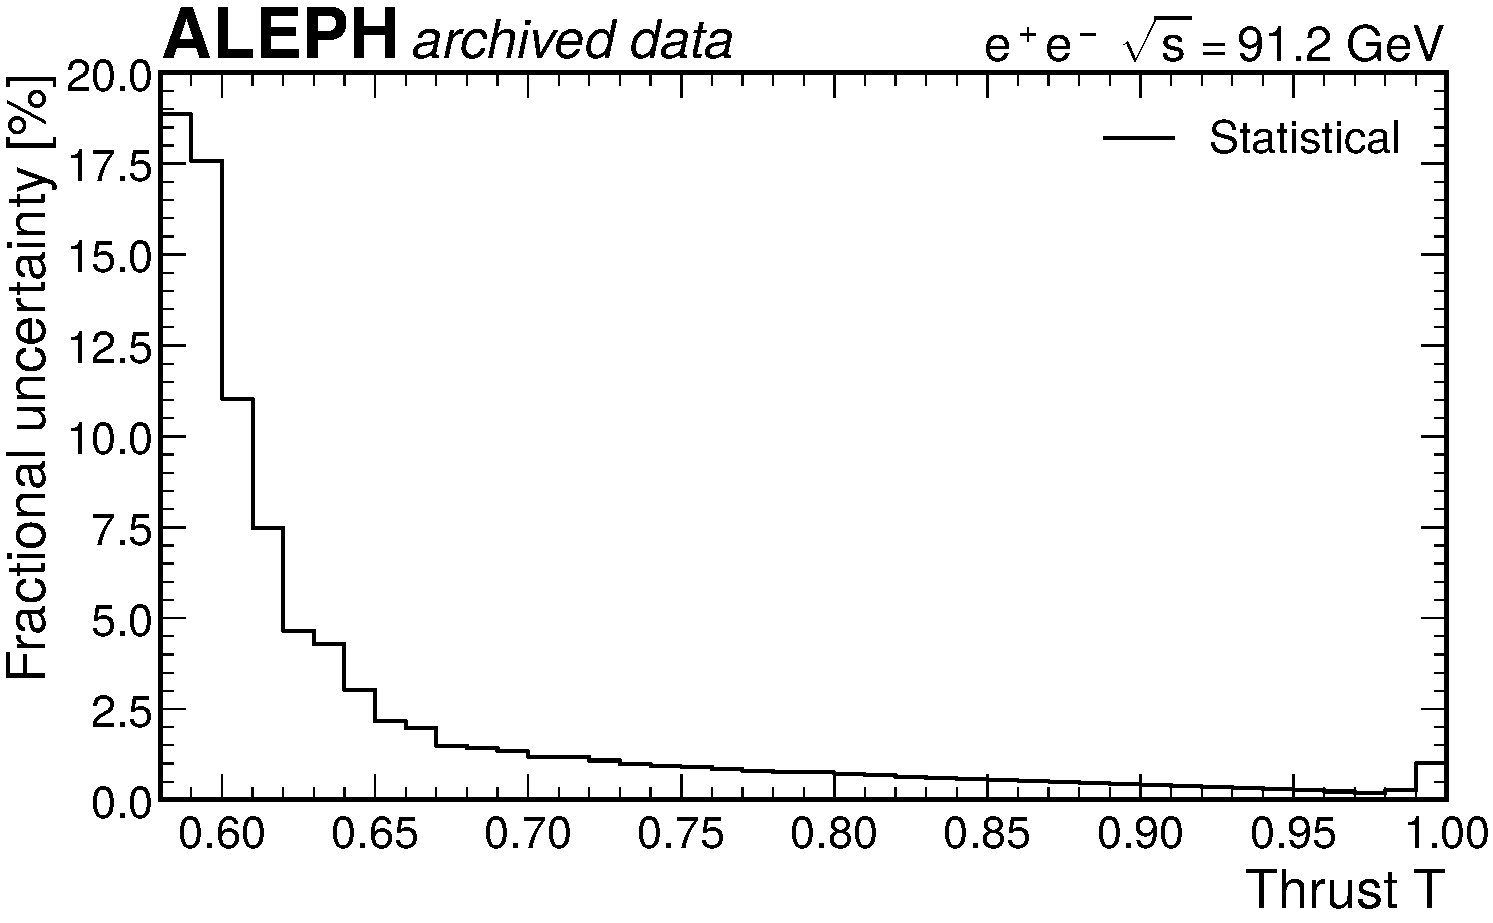
\includegraphics[width=0.49\textwidth]{figures/uncertainty_components_statistical.pdf}%
\hfill%
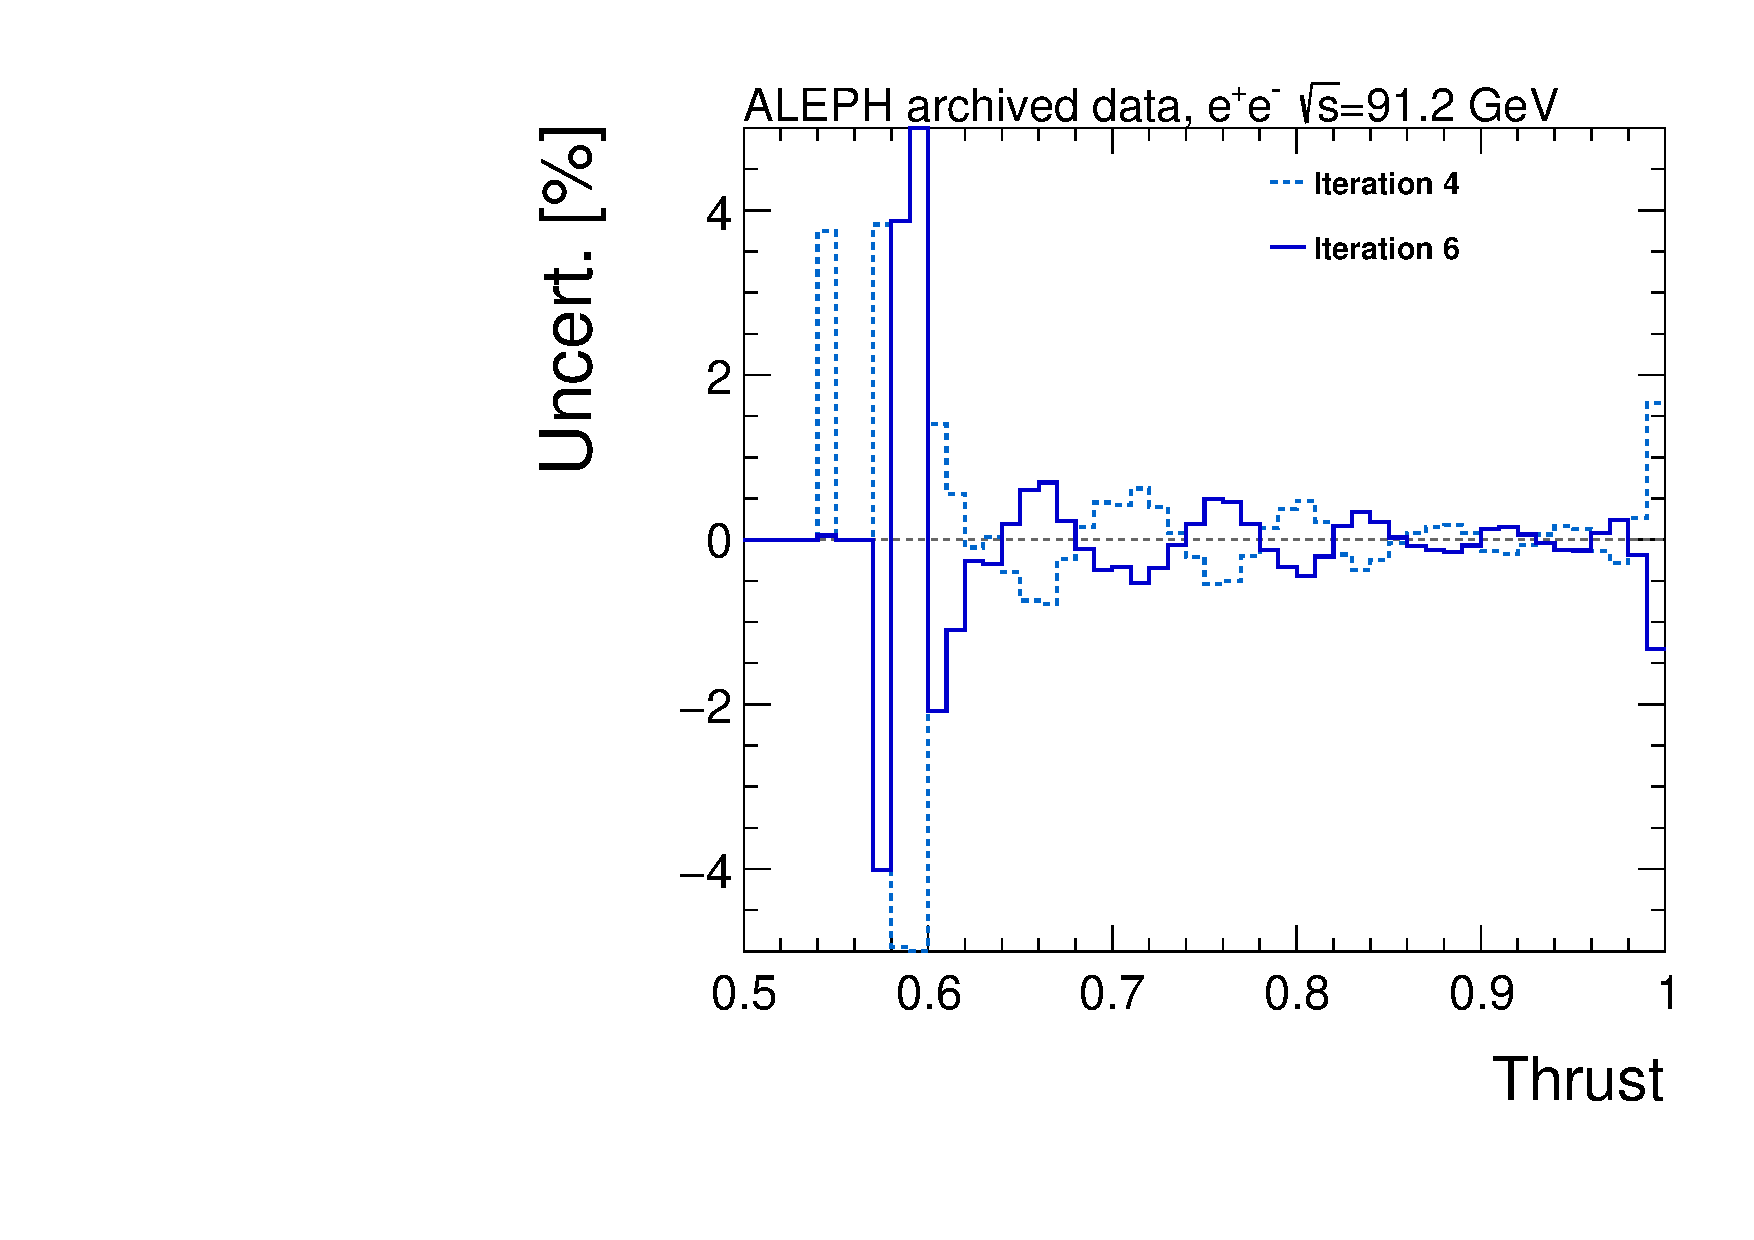
\includegraphics[width=0.49\textwidth]{figures/uncertainty_components_unfolding.pdf}
\caption{Signed per-bin shifts for the statistical (left) and unfolding-iteration
(right) uncertainty components. The statistical component is nearly flat and small
across the spectrum. The iteration panel shows $N_{\mathrm{iter}}=4$ and $6$
relative to the nominal $N_{\mathrm{iter}}=5$.}
\label{fig:unc_comp_stat_iter}
\end{figure}

\FloatBarrier

\subsection{Experimental systematic uncertainties}
\label{sec:exp_systematics}

Experimental systematic uncertainties are handled following the standard ALEPH procedure~\cite{Heister:2003aj} to vary individual selections, rerunning the full analysis chain, and measuring the difference with respect to the nominal as the uncertainty. The systems are defined below. The experimental subtotal and the final total are formed by quadrature of their sub-components.

\begin{itemize}
  \item \texttt{iter4}/\texttt{iter6}: unfolding passes at $N_{\mathrm{iter}}=4$ and $6$.
  \item \texttt{ntpc7}: tightened TPC hit requirement ($N_{\mathrm{TPC}}>7$, nominal $>4$).
  \item \texttt{pt04}: raised charged-$p_T$ threshold ($>0.4$~GeV, nominal $>0.2$~GeV).
  \item \texttt{ech10}: loosened charged-energy cut ($>10$~GeV, nominal $>15$~GeV).
  \item \texttt{with\_met}: missing transverse energy added as a pseudo-particle.
  \item \texttt{nes\_up}/\texttt{nes\_down}: neutral energies scaled up and down, probing ECAL energy-scale uncertainty.
  \item \texttt{ner}: neutral objects randomly removed, probing reconstruction efficiency.
\end{itemize}

Figure~\ref{fig:unc_comp_exp} shows the signed per-bin shifts for all variations. The largest contributions arise at low thrust ($T\lesssim 0.62$) where the steeply rising spectrum amplifies small absolute shifts; across the central range the experimental envelope is at the few-percent level.

\begin{figure}[ht!]
\centering
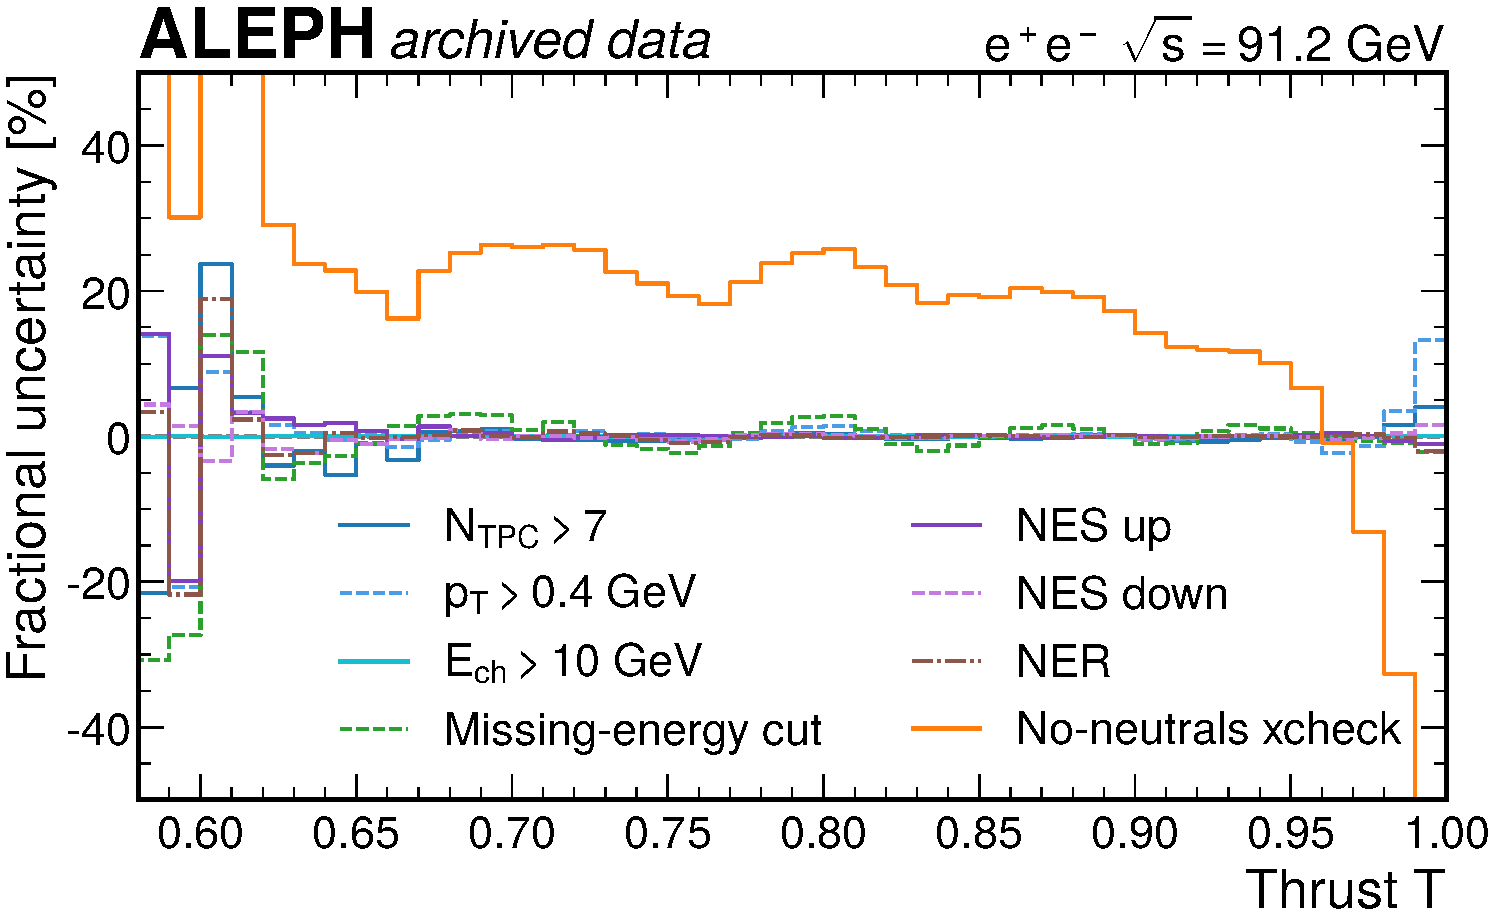
\includegraphics[width=0.85\textwidth]{figures/uncertainty_components_experimental.pdf}
\caption{Signed per-bin shifts for the seven experimental variation branches: the four
track/event branches (\texttt{ntpc7}, \texttt{pt04}, \texttt{ech10},
\texttt{with\_met}) and the three neutral-response branches (\texttt{nes\_up},
\texttt{nes\_down}, \texttt{ner}). The \texttt{no\_neutrals} curve is a cross-check and
does not enter the uncertainty.}
\label{fig:unc_comp_exp}
\end{figure}

The neutral-object response variations are chosen in preference to the standard ALEPH approach of removing all neutral particles within 1-2 GeV from the event~\cite{Heister:2003aj}. The reason is that
removing neutrals entirely redefines the observable: the resulting distribution is no longer the energy-flow thrust $T_{\mathrm{EF}}$ but a different quantity, charged-only thrust $T_{\mathrm{ch}}$, computed from a different particle-level definition. Treating the difference $T_{\mathrm{EF}} - T_{\mathrm{ch}}$ as a systematic uncertainty on the energy-flow measurement would conflate two distinct observables and produce an uncertainty that is unphysically large. Instead, \texttt{nes\_up}, \texttt{nes\_down}, and \texttt{ner} vary the detector response to neutral objects while holding the particle-level definition fixed, providing a physically meaningful probe of calorimeter modeling uncertainties without changing
what is being measured.

To quantify this distinction, the full unfolding chain was repeated with neutral particles ($\mathrm{pwflag}\in\{4,5\}$) removed, yielding a charged-only thrust distribution as shown in Figure~\ref{fig:charged_vs_ef}. Both the energy-flow and charged-only results are processed through the complete analysis chain. The reconstructed particle collection differs between the two, but both are unfolded to the same energy-flow particle-level definition. Both distributions are shown with statistical uncertainties only; the full systematic suite is not propagated for this diagnostic comparison, and the charged-only branch is excluded from the nominal total uncertainty combination. The charged-only spectrum is systematically broader than the energy-flow, as expected from the missing neutral-energy deposits. In the central range the mean shift is approximately $23\%$.

\begin{figure}[t!]
\centering
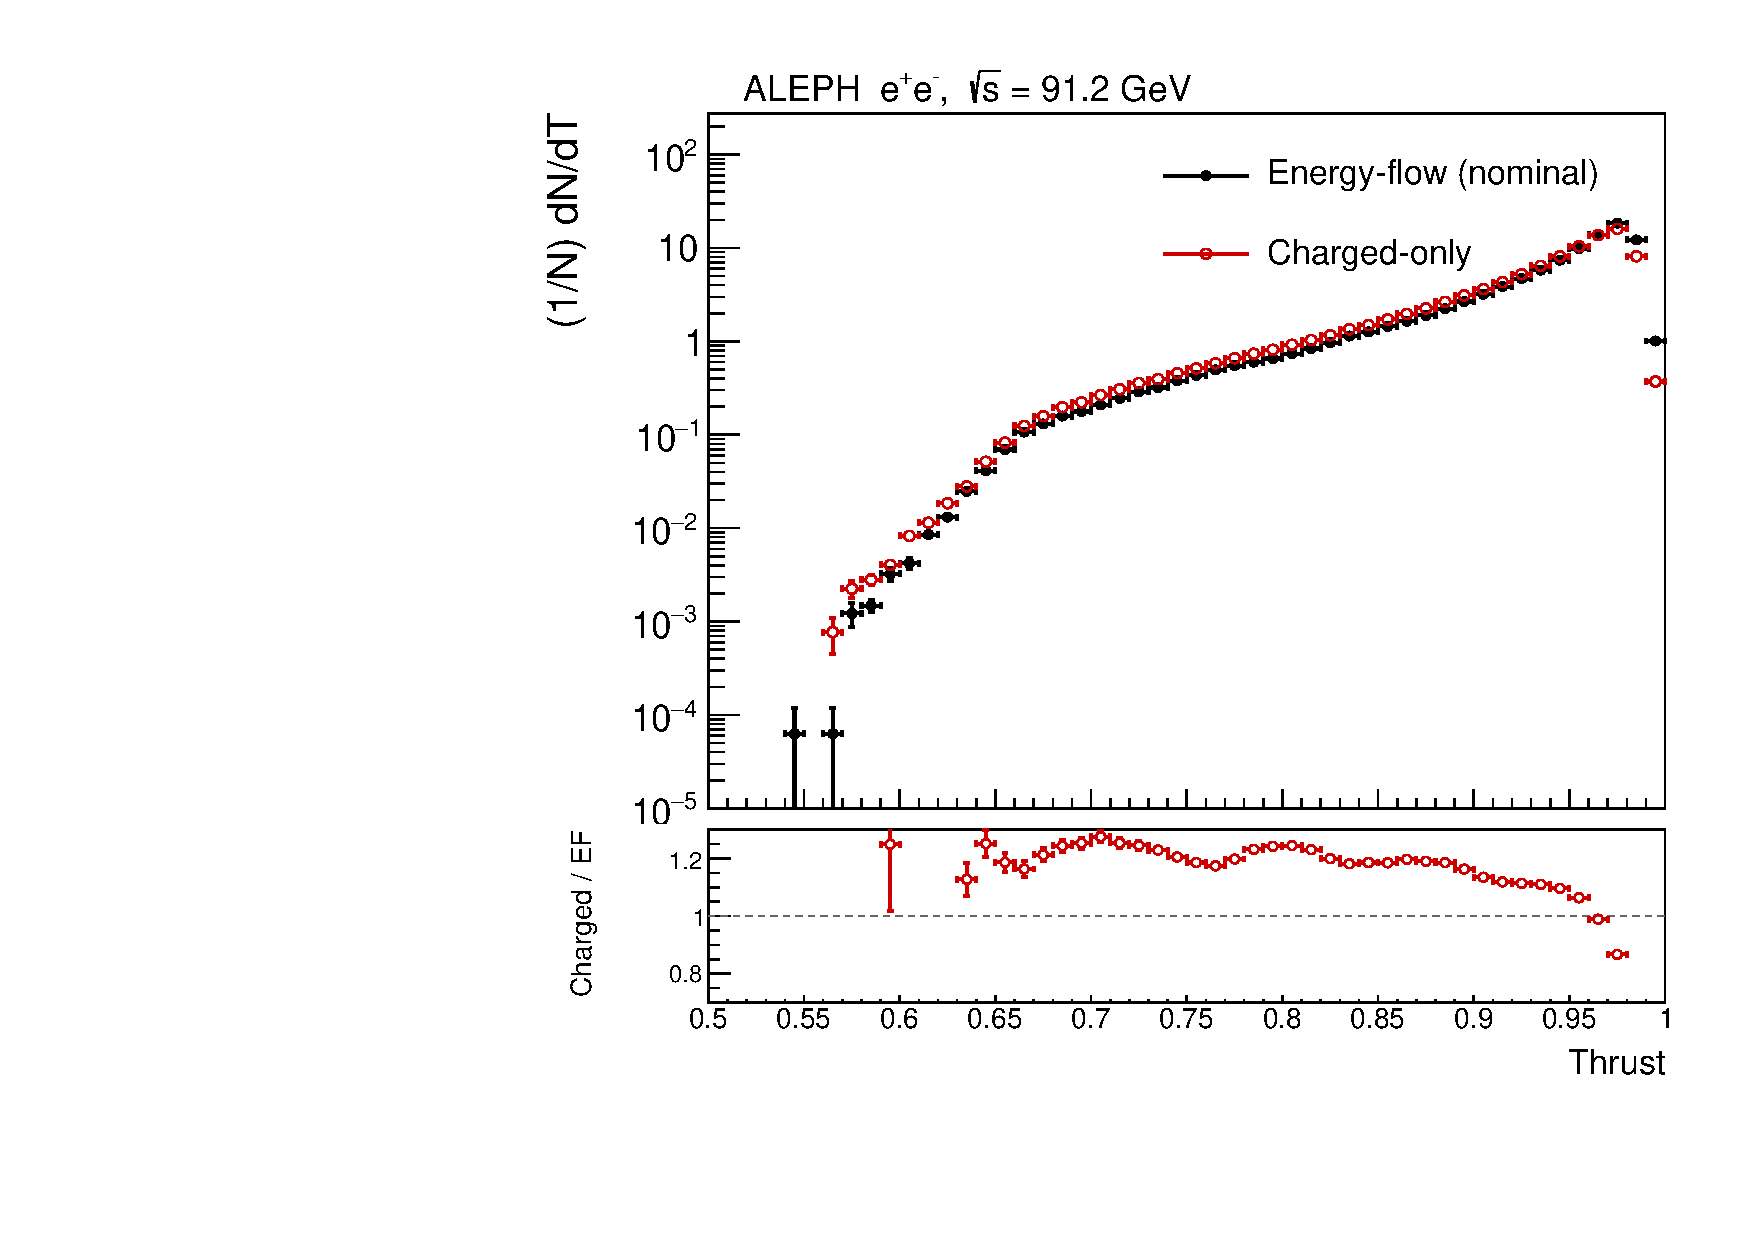
\includegraphics[width=0.70\textwidth]{figures/charged_only_vs_energy_flow.pdf}
\caption{Comparison of the charged-only (red open circles) and energy-flow (black filled circles) unfolded thrust distributions. Error bars represent statistical uncertainties only.}
\label{fig:charged_vs_ef}
\end{figure}

The track and neutral object variations are combined as described below. The full experimental envelope is then combined in quadrature.

\begin{align}
\Delta_{\mathrm{track/event}}(j) &=
  \sqrt{\sum_{v\in\{\mathrm{ntpc7,\,pt04,\,ech10,\,with\_met}\}} |\delta_v(j)|^2}. \\
  \Delta_{\mathrm{neutral}}(j) & =
\sqrt{\max\!\left(|\delta_{\mathrm{nes\_up}}(j)|,|\delta_{\mathrm{nes\_down}}(j)|\right)^2
    + |\delta_{\mathrm{ner}}(j)|^2}. \\ 
\Delta_{\mathrm{exp}}(j) &= \sqrt{\Delta_{\mathrm{track/event}}^2(j)+\Delta_{\mathrm{neutral}}^2(j)}.
\end{align}

\FloatBarrier

\subsection{Theory systematic uncertainties}
\label{sec:theory_systematics}

Theory systematic variations probe the residual model dependence introduced by the Monte Carlo generator used in the unfolding. The nominal response matrix is constructed from \textsc{Pythia}~6~\cite{Sjostrand:2000wi}, the ALEPH simulation. Three additional generators are used to reweight the generator-level thrust distribution event-by-event, producing alternative response matrices that span a
wide range of parton-shower algorithms and hadronization models: \textsc{Pythia}~8.317 with Monash tune, dipole-ordered shower~\cite{Bierlich:2022pfr}, \textsc{Herwig}~7.1.5, angular-ordered shower with cluster hadronization~\cite{B_hr_2008,Bellm:2015jjp,Bellm:2017bvx, bewick2024herwig73releasenote}, and \textsc{Sherpa}~2.2.6 with AHADIC++ hadronization~\cite{Bothmann2019}.
The theory envelope is taken as the maximum absolute shift across the three generators:
\begin{equation}
\Delta_{\mathrm{theory}}(j)=
  \max\!\left(|\delta_{\mathrm{pythia8}}(j)|,
             |\delta_{\mathrm{herwig}}(j)|,
             |\delta_{\mathrm{sherpa}}(j)|\right).
\end{equation}
The three generators diverge progressively at lower thrust, where multi-jet configurations and hard, wide-angle gluon emission dominate and the parton-shower and matrix-element matching differ between generators; there the reweighted
generator-level spectra move coherently and by similar amounts. The envelope also rises in the last bin, $0.99\le T<1.00$, where the reweighted spectra are least well constrained: the bin sits at the edge of the two-jet limit, and the shift there is not smoothly connected to its neighbours. The theory envelope is the dominant uncertainty contribution across the central measurement range, as shown in Figure~\ref{fig:unc_comp_theory}.

\begin{figure}[ht!]
\centering
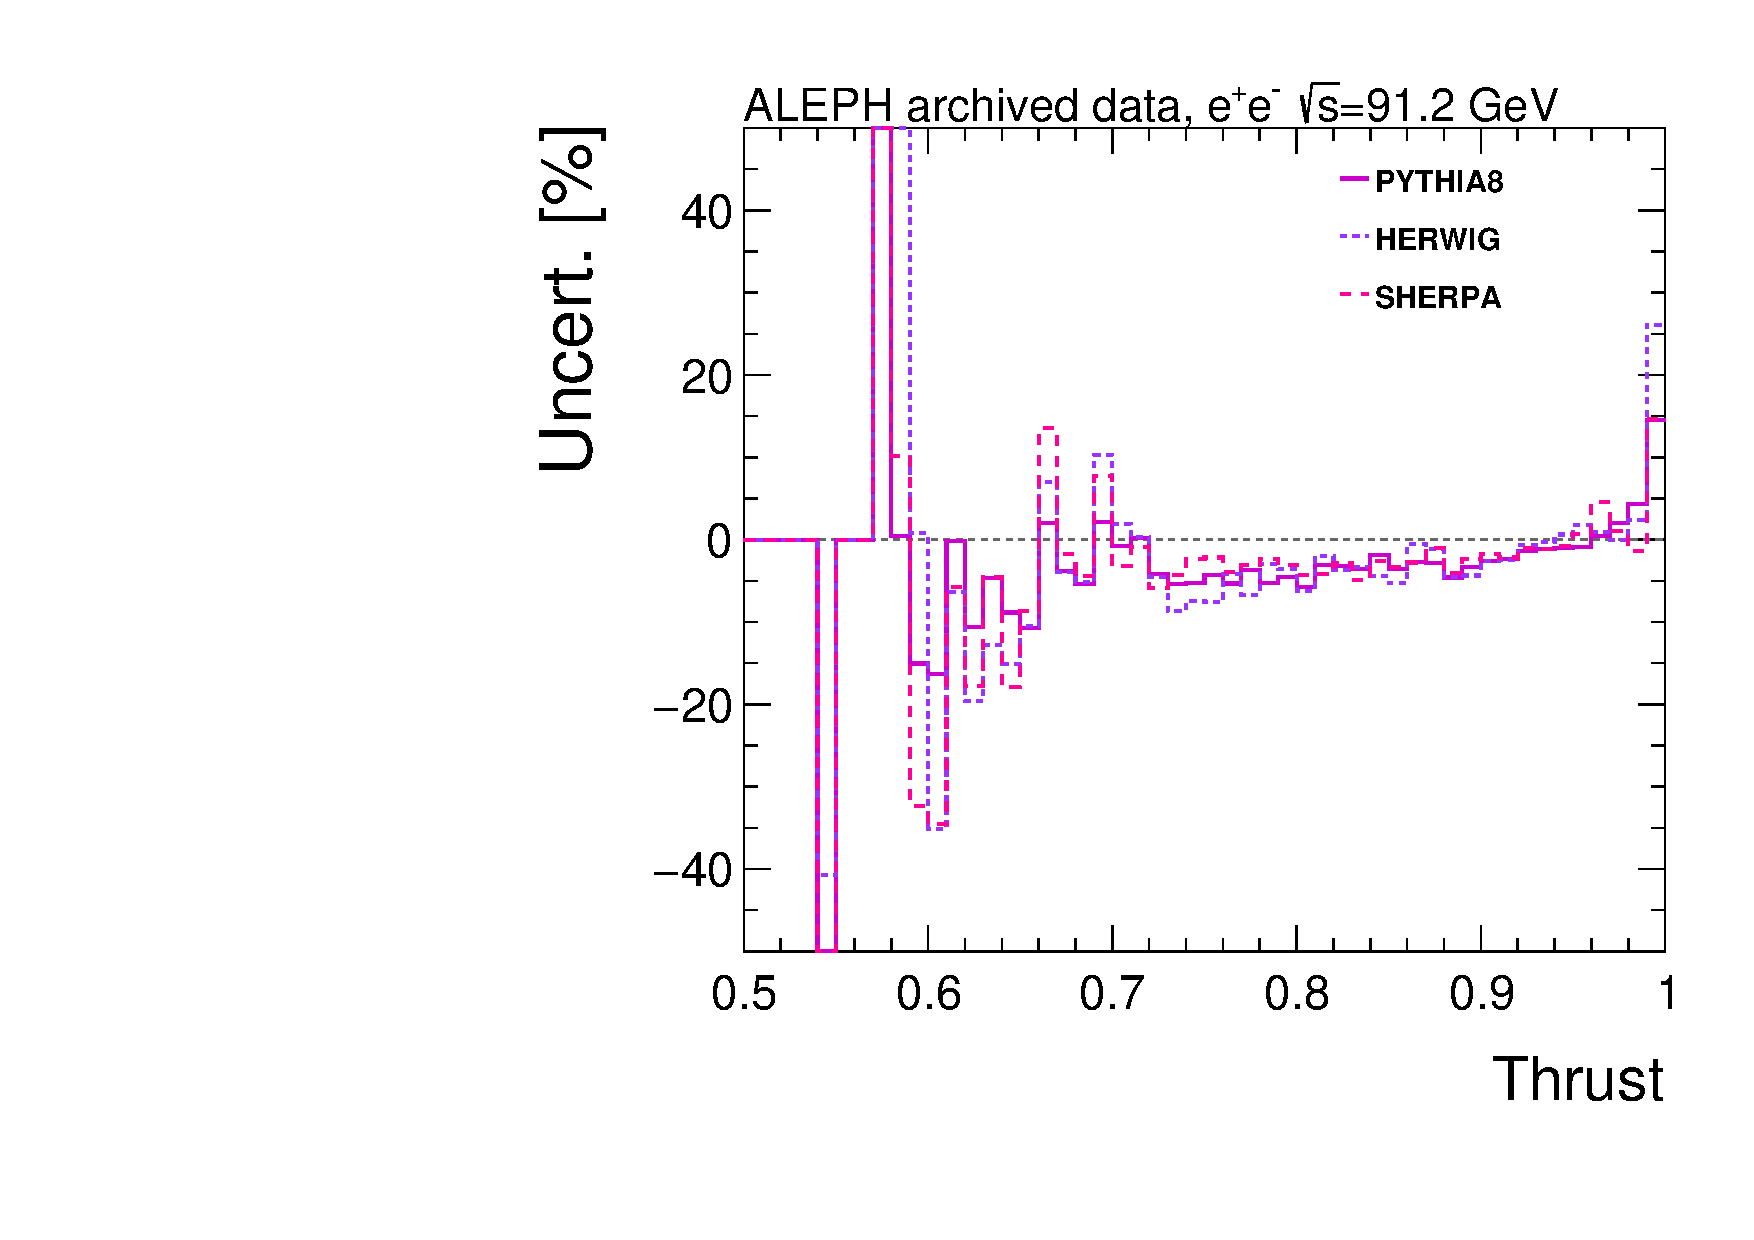
\includegraphics[width=0.85\textwidth]{figures/uncertainty_components_theory.pdf}
\caption{Signed per-bin shifts for the theory prior variations from \textsc{Pythia}~8.317, \textsc{Herwig}~7.1.5, and \textsc{Sherpa}~2.2.6.}
\label{fig:unc_comp_theory}
\end{figure}

\FloatBarrier

\subsection{Hadronic event-selection correction}
\label{sec:had_uncertainty}

After unfolding, a bin-wise hadronic event-selection correction is applied to account for the fraction of hadronic events lost to the generator-level selection:
\begin{equation}
C_{\mathrm{had}}(j) = \frac{N_{\mathrm{genBefore}}(j)}{N_{\mathrm{gen}}(j)},
\qquad
U_j^{\mathrm{corr}} = U_j\,C_{\mathrm{had}}(j).
\end{equation}
This correction maps the unfolded spectrum from the generator-level hadronic-event-selected phase space to the full inclusive hadronic phase space. The uncertainty on this correction is propagated as an independent component
$\Delta_{\mathrm{had}}$. The correction is computed from two generator-level histograms: \texttt{tgenBefore} (events before hadronic selection) and \texttt{tgen} (events passing hadronic selection). Statistical uncertainties on both histograms are propagated through the ratio using standard error propagation, yielding symmetric bin-wise up and down variations $C_{\mathrm{had}}^{\pm}(j)$. These variations are applied to the unfolded spectrum and normalized to the differential cross-section basis, producing up and down shifted spectra. 

% The fractional hadronic correction uncertainty is then defined as the envelope:
% \begin{equation}
% \delta_{\mathrm{had}}^{\pm}(j) = \frac{U_j \cdot C_{\mathrm{had}}^{\pm}(j) / \int U \cdot C_{\mathrm{had}}^{\pm}\,dT}{U_j^{\mathrm{corr}}} - 1,
% \end{equation}
% with $\Delta_{\mathrm{had}}(j) = \max(|\delta_{\mathrm{had}}^{+}(j)|, |\delta_{\mathrm{had}}^{-}(j)|)$.

\subsection{QED ISR correction}
\label{sec:isr_uncertainty}

The QED ISR correction removes the contribution of events
where the $e^+e^-$ center-of-mass energy is reduced by photon radiation before the hard scatter, mapping the measured distribution from the ISR-inclusive sample
to the pure $\sqrt{s}=M_Z$ distribution:
\begin{equation}
C_{\mathrm{ISR}}(j) = \frac{N^{\mathrm{gen}}_{\mathrm{no\,ISR}}(j)}{N^{\mathrm{gen}}_{\mathrm{ISR}}(j)}.
\end{equation}
Both published ALEPH event-shape analyses apply this
correction~\cite{Barate:1996fi,Heister:2003aj}. The 1998 ALEPH analysis~\cite{Barate:1996fi} defines it as the ratio of generator-level thrust distributions produced with and without ISR, using \textsc{JETSET}~7.4. The 2004 analysis~\cite{Heister:2003aj} uses \textsc{KORALZ}, which provides a more accurate treatment of ISR, to generate the corrected distribution.

The ISR correction is applied bin-by-bin after the hadronic correction using standalone \textsc{Pythia}~8.317 samples with ISR disabled (\texttt{isr0}) and enabled (\texttt{isr1}), as described in Sec.~\ref{sec:corrections_and_cov}. The uncertainty on
this correction is derived from the finite Monte Carlo statistics. Up and down variations $C_{\mathrm{ISR}}^{\pm}(j) = C_{\mathrm{ISR}}(j)\cdot(1\pm\sigma_{\mathrm{rel}}(j))$ are applied to the unfolded spectrum and the envelope is taken as $\Delta_{\mathrm{ISR}}(j)$. The uncertainty is purely MC-statistical in nature for simplicity, but should be assessed in closer detail for future work. 

% The \textsc{Pythia}~8.317 generator used here gives a less accurate ISR description than the \textsc{KORALZ} generator used in the ALEPH 2004 analysis~\cite{Heister:2003aj}; for a full measurement the modern equivalent, \textsc{KKMCee}~5.00.02, would be the natural choice, as noted in Sec.~\ref{sec:corrections_and_cov}.

\subsection{Covariance evaluation}
\label{sec:stat_covariance}

For the nominal run, the statistical covariance is computed by RooUnfold using analytical error propagation (\texttt{RooUnfold::kCovariance}), which propagates
Poisson uncertainties in the data and response histograms through the IBU iteration chain without toy MC sampling. The resulting covariance matrix is read from the unfolding output and transformed to the normalized differential-thrust basis used in this work.

Non-statistical component covariances are built with a configurable model. The current nominal release uses the \texttt{template\_correlated} option, where each non-statistical component covariance is built as
\begin{equation}
\mathrm{Cov}^{(c)}_{ij}=\Delta_c(i)\,\Delta_c(j)\,\rho^{\mathrm{stat}}_{ij},
\end{equation}
with $\rho^{\mathrm{stat}}_{ij}$ taken from the statistical unfolding covariance correlation template. This keeps component magnitudes tied to the measured per-bin
shifts while avoiding a purely diagonal systematic-covariance approximation. For cross-check studies, \texttt{diagonal} and \texttt{block} component models
are also available~\cite{Adye:2011gm}.

\subsection{Combination model}
\label{sec:combination_model}

The total bin uncertainty combines all seven components in quadrature:
\begin{equation}
\Delta_{\mathrm{tot}}(j)=\sqrt{\Delta_{\mathrm{stat}}^2(j)
+ \Delta_{\mathrm{iter}}^2(j) + \Delta_{\mathrm{exp}}^2(j)
+ \Delta_{\mathrm{theory}}^2(j) + \Delta_{\mathrm{had}}^2(j)
+ \Delta_{\mathrm{ISR}}^2(j)}.
\end{equation}
The quadrature sum is used since the components originate from distinct sources and the covariance cross terms are expected to be small.

\subsection{Uncertainty breakdown}
\label{sec:uncertainty_breakdown}

Figure~\ref{fig:per_bin_uncertainty_grid} shows the absolute fractional uncertainties. Theory is the dominant source across the central range, where the experimental envelope is smaller by roughly a factor of two. The statistical and iteration components remain sub-percent in the bulk.

\begin{figure}[ht!]
\centering
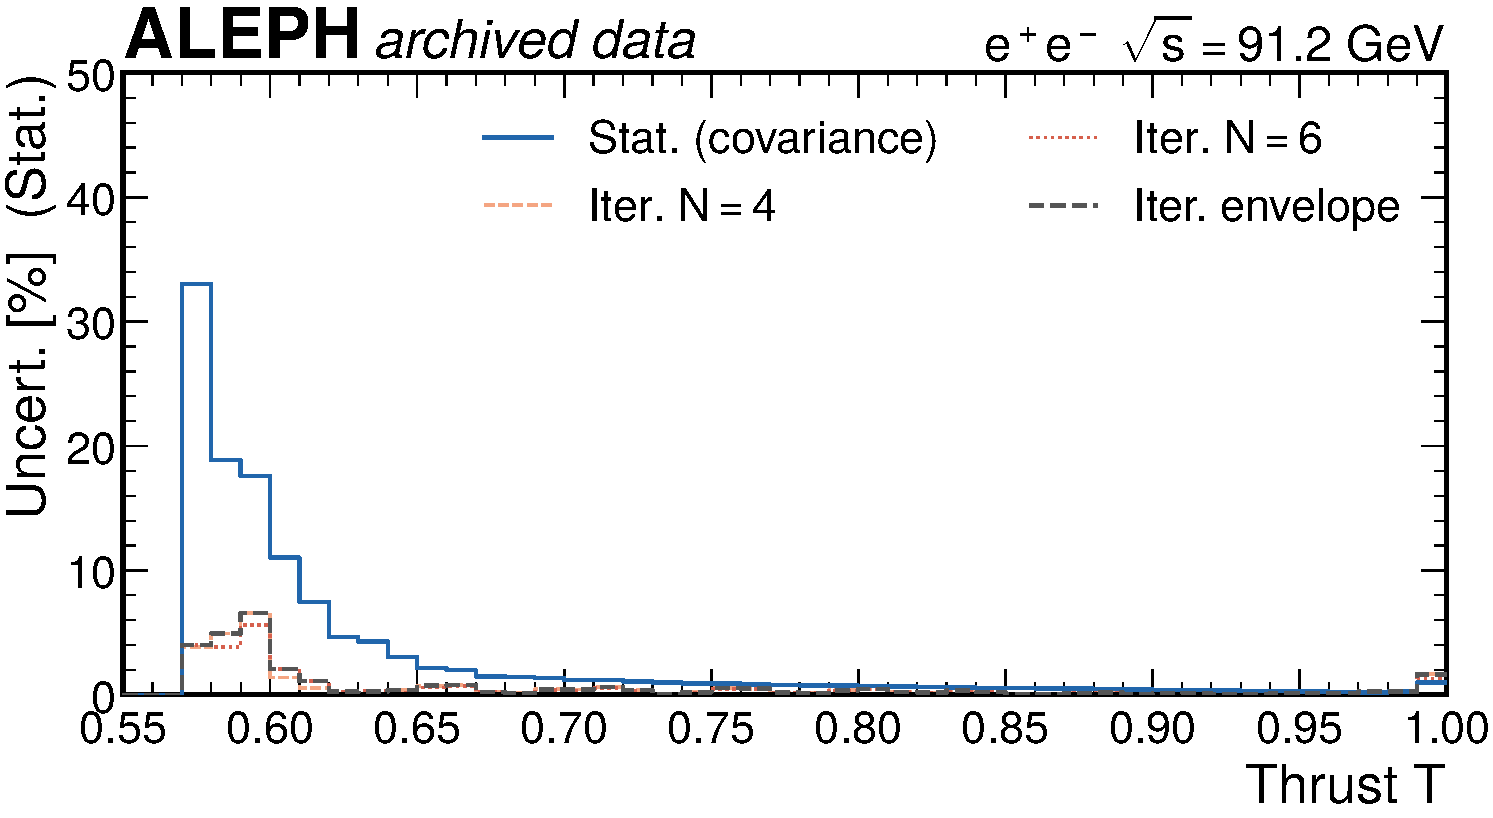
\includegraphics[width=0.49\textwidth]{figures/per_bin_uncertainty_stat.pdf}%
\hfill%
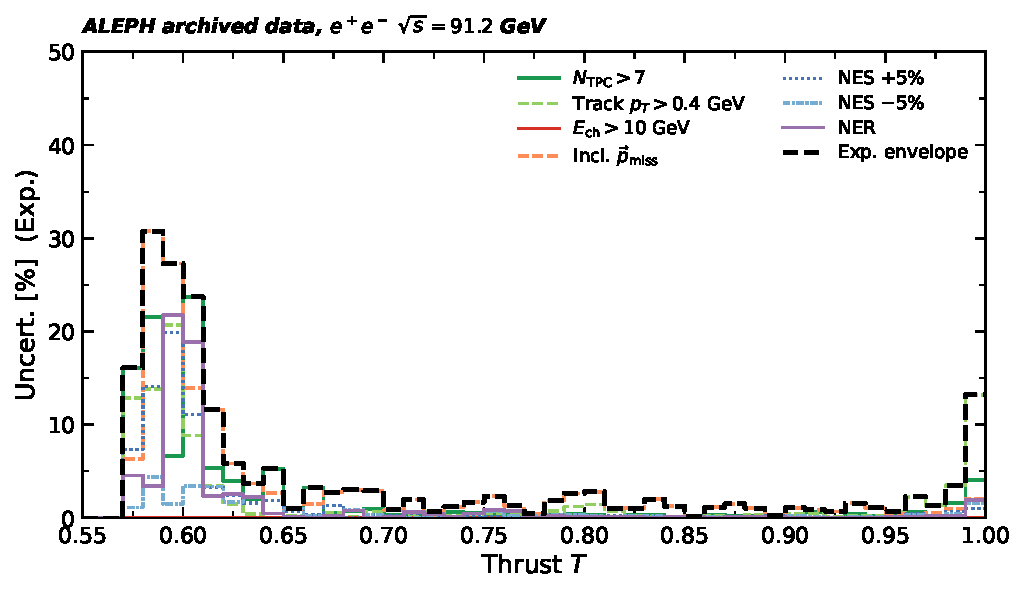
\includegraphics[width=0.49\textwidth]{figures/per_bin_uncertainty_exp.pdf}\\[2mm]
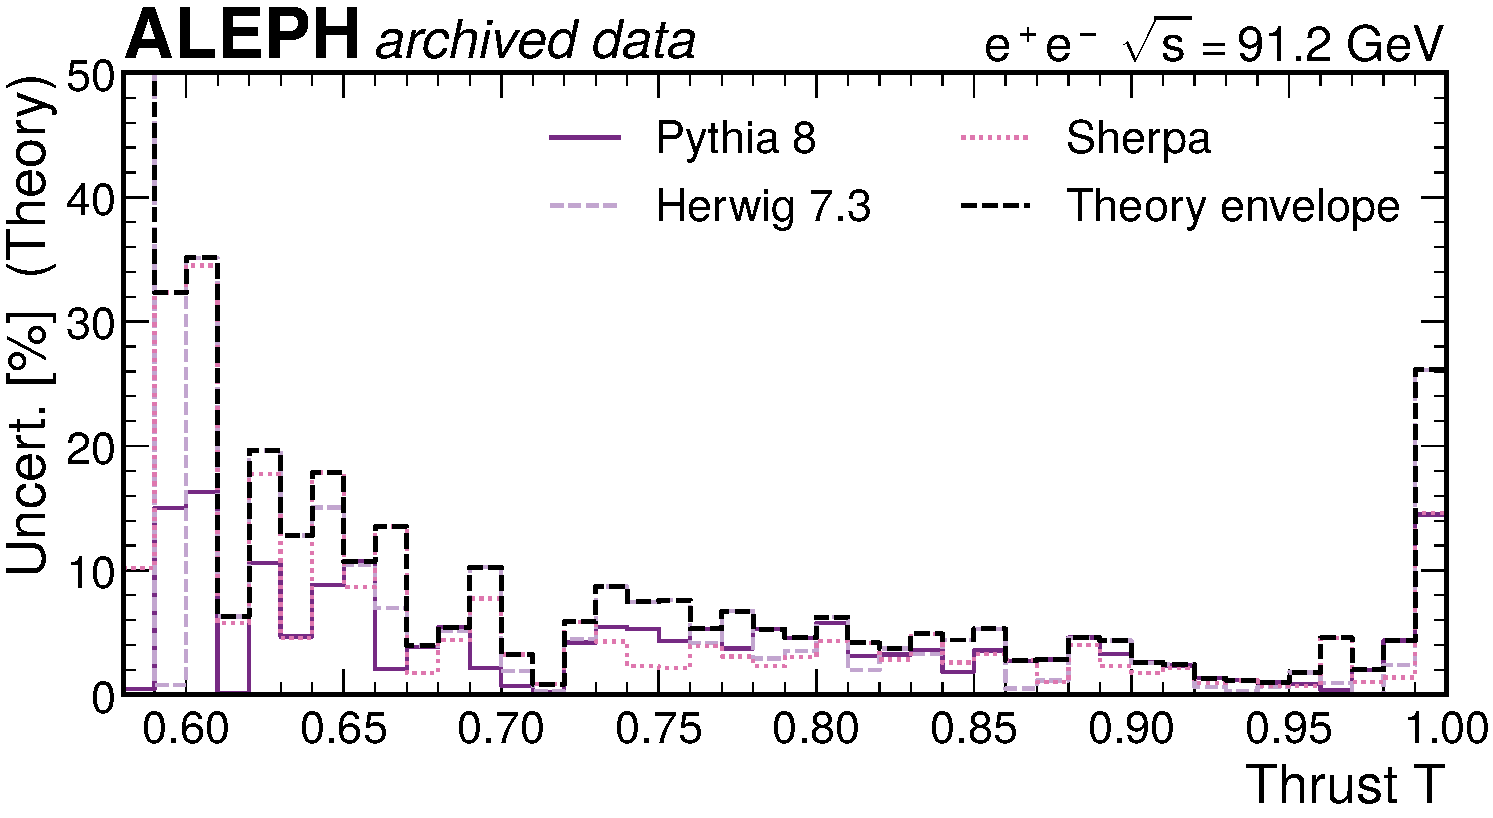
\includegraphics[width=0.49\textwidth]{figures/per_bin_uncertainty_theory.pdf}%
\hfill%
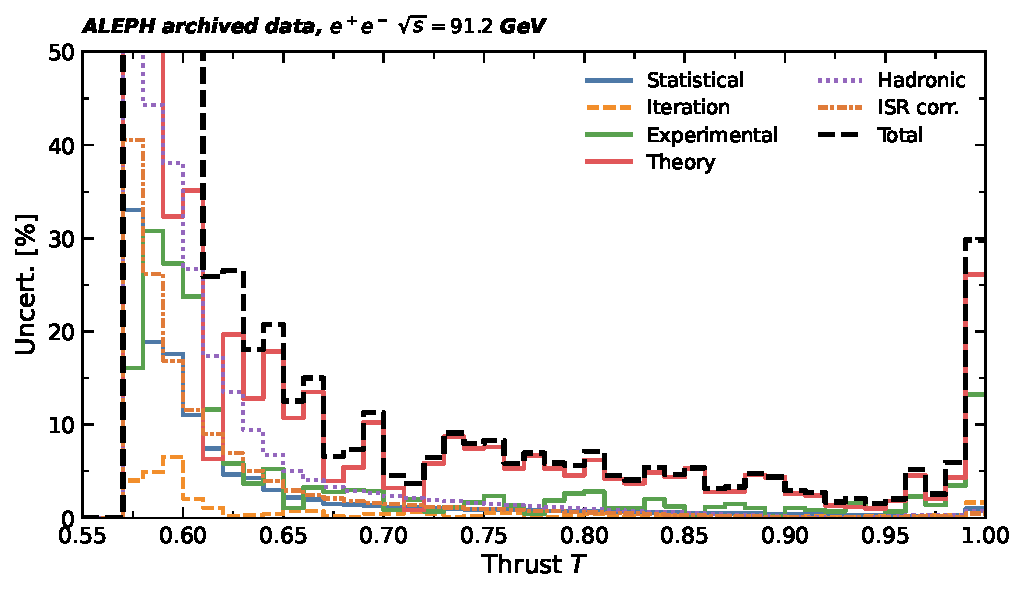
\includegraphics[width=0.49\textwidth]{figures/per_bin_uncertainty_grouped.pdf}
\caption{Fractional uncertainties: (top left) statistical and unfolding-iteration components, (top right) experimental variation branches with group envelope, (bottom left) theory reweighting branches with theory envelope, (bottom right) all groups overlaid.
%The neutral energy-scale branches respond non-linearly to a symmetric variation, so their up and down shifts differ at low thrust while agreeing across the reported range. The charged-$p_T$ branch peaks in the last bin, where removing soft tracks migrates events against the kinematic boundary.
}
\label{fig:per_bin_uncertainty_grid}
\end{figure}

